% !TeX program = xelatex
\documentclass[a4paper,10pt]{article}

% ============================================================================
% កញ្ចប់បណ្ណាល័យ (Packages) – តាមលំនាំ NGS Preah Krasang (ls_plan.tex)
% បរិបទ៖ គ្មានស្លាយ LCD — ប្រើក្ដារខៀន + សន្លឹកកិច្ចការសិស្ស ស-ខ្មៅ ជាគោល
% ============================================================================
\usepackage[a4paper, left=0.95cm, right=0.95cm, top=0.85cm, bottom=0.92cm, footskip=0.52cm]{geometry}
\usepackage{amsmath}
\usepackage{unicode-math}
\usepackage{fontspec}
\usepackage{array, longtable, multirow, colortbl}
\usepackage[table]{xcolor}
\usepackage{enumitem}
\usepackage{pifont}
\usepackage{fancyhdr}
\usepackage{tikz}
\usetikzlibrary{calc, arrows.meta, angles, quotes, decorations.markings, babel}

% LaTeX 2025 + longtable compatibility guard
\makeatletter
\let\@expl@@@mark@update@singlecol@structures@@\relax
\makeatother

% ============================================================================
% ការកំណត់ពុម្ពអក្សរ (Cross-Platform Fonts Configuration)
% ============================================================================
\providecommand{\NGSFindFonts}{%
  \IfFileExists{C:/Windows/Fonts/cambria.ttc}{%
    \def\NGSSysPath{C:/Windows/Fonts/}%
    \def\NGSUserPath{C:/Users/KIT/AppData/Local/Microsoft/Windows/Fonts/}%
  }{%
    \IfFileExists{./fonts/KhmerOSsiemreap.ttf}{\def\NGSSysPath{./fonts/}\def\NGSUserPath{./fonts/}}{%
    \IfFileExists{../fonts/KhmerOSsiemreap.ttf}{\def\NGSSysPath{../fonts/}\def\NGSUserPath{../fonts/}}{%
    \IfFileExists{../../fonts/KhmerOSsiemreap.ttf}{\def\NGSSysPath{../../fonts/}\def\NGSUserPath{../../fonts/}}{%
    \IfFileExists{../../../fonts/KhmerOSsiemreap.ttf}{\def\NGSSysPath{../../../fonts/}\def\NGSUserPath{../../../fonts/}}{%
    \IfFileExists{../../../../fonts/KhmerOSsiemreap.ttf}{\def\NGSSysPath{../../../../fonts/}\def\NGSUserPath{../../../../fonts/}}{%
    \IfFileExists{../../../../../fonts/KhmerOSsiemreap.ttf}{\def\NGSSysPath{../../../../../fonts/}\def\NGSUserPath{../../../../../fonts/}}{%
    \IfFileExists{../../../../../../fonts/KhmerOSsiemreap.ttf}{\def\NGSSysPath{../../../../../../fonts/}\def\NGSUserPath{../../../../../../fonts/}}{%
      \def\NGSSysPath{../../../../../../../fonts/}\def\NGSUserPath{../../../../../../../fonts/}%
    }}}}}}}%
  }%
}
\NGSFindFonts

\setmathfont[
  Path={\NGSSysPath},
  FontIndex=1,
  Scale=1.02
]{cambria.ttc}

\defaultfontfeatures{Ligatures=TeX}

\setmainfont[
  Path={\NGSUserPath},
  Extension=.ttf,
  Script=Khmer,
  BoldFont={KhmerOSsiemreap},
  BoldFeatures={FakeBold=1.8},
  ItalicFont={KhmerOSsiemreap},
  ItalicFeatures={FakeSlant=0.25},
  BoldItalicFont={KhmerOSsiemreap},
  BoldItalicFeatures={FakeBold=1.8, FakeSlant=0.25}
]{KhmerOSsiemreap}

\newfontfamily\muol[
  Path={\NGSUserPath},
  Extension=.ttf,
  Script=Khmer
]{KhmerOSmuollight}

\newfontfamily\TimesEn[
  Path={\NGSSysPath},
  Extension=.ttf,
  Scale=1.00,
  BoldFont={timesbd},
  ItalicFont={timesi},
  BoldItalicFont={timesbi}
]{times}

\newfontfamily\NagaBold[
  Path={\NGSUserPath},
  Extension=.ttf
]{AKbalthom Naga Bold}

\newfontfamily\CalibriFont[
  Path={\NGSSysPath},
  Extension=.ttf
]{calibri}

\newfontfamily\Tacteing[
  Path={\NGSUserPath}
]{TACTENG.TTF}

\newfontfamily\CourierBullet[
  Path={\NGSSysPath},
  Extension=.ttf
]{cour}
\newcommand{\wcirc}{{\CourierBullet\fontsize{9.5pt}{11pt}\selectfont o}}

\XeTeXlinebreaklocale "km"
\XeTeXlinebreakskip = 0pt plus 1pt minus 0.1pt

% ============================================================================
% ការកំណត់ពណ៌ និងទម្រង់ទំព័រ (Colors & Page Style)
% ============================================================================
\definecolor{stepgray}{HTML}{D9D9D9}
\definecolor{headgray}{HTML}{F2F2F2}
\definecolor{boxgray}{HTML}{D9D9D9}
\definecolor{darkred}{HTML}{C00000}
\definecolor{red5e}{HTML}{FF0000}

\pagestyle{fancy}
\fancyhf{}
\renewcommand{\headrulewidth}{0pt}
\fancyfoot[R]{\CalibriFont\fontsize{11pt}{13pt}\selectfont\thepage}

\setlength{\parindent}{0pt}
\setlength{\parskip}{0pt}
\setlength{\tabcolsep}{3.8pt}

\newcolumntype{L}[1]{>{\raggedright\arraybackslash}p{#1}}

% ============================================================================
% ម៉ាក្រូជំនួយ (Helper Macros)
% ============================================================================
\newcommand{\en}[1]{{\TimesEn #1}}
\newcommand{\enbf}[1]{{\TimesEn\textbf{#1}}}
\newcommand{\unit}[1]{\,\text{\en{#1}}}
\newcommand{\fiveE}[1]{{\NagaBold\fontsize{9.5pt}{13pt}\selectfont\textcolor{red5e}{#1}}}
\newcommand{\timenote}[1]{\textcolor{darkred}{\textit{#1}}}
\newcommand{\redsub}[1]{\textcolor{darkred}{#1}}
\newcommand{\graybox}[1]{\colorbox{boxgray}{\strut\hspace{2pt}#1\hspace{2pt}}}
\newcommand{\ditem}{\tikz[baseline=-0.5ex]\fill (0,0.42ex) -- (0.42ex,0) -- (0,-0.42ex) -- (-0.42ex,0) -- cycle;\hspace{0.3em}}
\newcommand{\cnum}[1]{{\fontsize{10.5pt}{12pt}\selectfont\ding{\numexpr181+#1\relax}}\hspace{0.2em}}
\newcommand{\cfig}[1]{\par\vspace{4pt}{\centering #1\par}\vspace{4pt}}
\newcommand{\stepheader}[1]{\multicolumn{3}{|c|}{\cellcolor{stepgray}\muol #1} \\* \noalign{\hrule height 0.4pt}}
\newcommand{\tri}[1]{\ensuremath{\triangle #1}}
\newcommand{\ang}[1]{\ensuremath{\angle #1}}
\newcommand{\khmflourish}{{\Tacteing\fontsize{36pt}{14pt}\selectfont\raisebox{-5pt}{3}}}

\tikzset{
  tk1/.style={postaction={decorate},decoration={markings,mark=at position 0.50 with {\draw[black, line width=0.85pt](0,-0.095)--(0,0.095);}}},
  tk2/.style={postaction={decorate},decoration={markings,
    mark=at position 0.45 with {\draw[black, line width=0.85pt](0,-0.095)--(0,0.095);},
    mark=at position 0.55 with {\draw[black, line width=0.85pt](0,-0.095)--(0,0.095);}}}
}

\newcommand{\rightbox}[4][0.18]{%
  \draw[black, line width=0.8pt]
    ($(#3)!#1!(#2)$) -- ($($(#3)!#1!(#2)$)+($(#3)!#1!(#4)$)-(#3)$) -- ($(#3)!#1!(#4)$);
}

% ============================================================================
% ម៉ាក្រូគូសរូបធរណីមាត្រ ស-ខ្មៅ (Proportional 4.0–7.0 cm, 100% Black Text)
% ============================================================================

% ១. រំលឹកលក្ខណៈមេដ្យាទ័រនៃអង្កត់ AB (MA = MB)
\newcommand{\figPrereqCIRC}{%
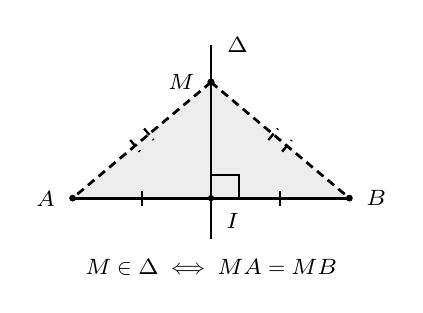
\begin{tikzpicture}[scale=0.95, every node/.style={font=\footnotesize, text=black}]
  \coordinate (A) at (-1.85,0);
  \coordinate (B) at (1.85,0);
  \coordinate (I) at (0,0);
  \coordinate (M) at (0,1.55);
  \coordinate (Top) at (0,2.05);
  \coordinate (Bot) at (0,-0.55);
  \fill[gray!14] (A) -- (M) -- (B) -- cycle;
  \draw[black, line width=1.05pt, tk1] (A) -- (I);
  \draw[black, line width=1.05pt, tk1] (I) -- (B);
  \draw[black, line width=0.95pt] (Bot) -- (Top) node[right=2pt] {$\Delta$};
  \draw[black, line width=1.0pt, densely dashed, tk2] (M) -- (A);
  \draw[black, line width=1.0pt, densely dashed, tk2] (M) -- (B);
  \rightbox[0.20]{M}{I}{B}
  \fill[black] (A) circle (1.3pt) node[left=2.5pt] {$A$};
  \fill[black] (B) circle (1.3pt) node[right=2.5pt] {$B$};
  \fill[black] (I) circle (1.2pt) node[below right=2pt] {$I$};
  \fill[black] (M) circle (1.4pt) node[left=3pt] {$M$};
  \node at (0,-0.92) {$M \in \Delta \iff MA = MB$};
\end{tikzpicture}}

% ២. E1 Engage: អណ្ដូងទឹករួមភូមិ ៣ (A, B, C មិនរត់ត្រង់ជួរ vs រត់ត្រង់ជួរ)
\newcommand{\figEngageCIRC}{%
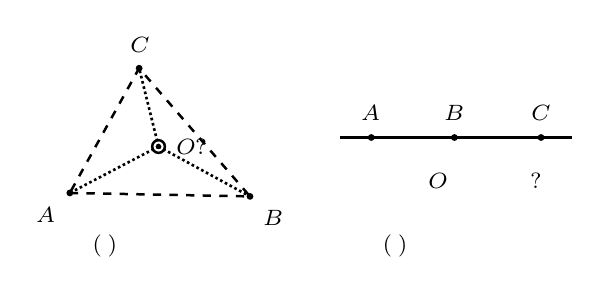
\begin{tikzpicture}[scale=0.88, every node/.style={font=\footnotesize, text=black}]
  % ខាងឆ្វេង៖ ភូមិ ៣ មិនរត់ត្រង់ជួរ
  \begin{scope}[shift={(0,0)}]
    \coordinate (A) at (0.25,0.25);
    \coordinate (B) at (2.85,0.20);
    \coordinate (C) at (1.25,2.05);
    \coordinate (O) at (1.53,0.92);
    \draw[black, line width=0.9pt, dashed] (A) -- (B) -- (C) -- cycle;
    \draw[black, line width=0.95pt, densely dotted] (O) -- (A) (O) -- (B) (O) -- (C);
    \fill[black] (A) circle (1.4pt) node[below left=1.5pt] {$A$};
    \fill[black] (B) circle (1.4pt) node[below right=1.5pt] {$B$};
    \fill[black] (C) circle (1.4pt) node[above=2pt] {$C$};
    \draw[black, line width=0.9pt] (O) circle (2.6pt);
    \fill[black] (O) circle (1.1pt) node[right=3pt] {$O?$};
    \node at (1.55,-0.52) {(ក) ភូមិ ៣ ជាត្រីកោណ};
  \end{scope}
  % ខាងស្ដាំ៖ ភូមិ ៣ រត់ត្រង់ជួរតាមផ្លូវជាតិ
  \begin{scope}[shift={(4.15,0)}]
    \draw[black, line width=1.05pt] (0,1.05) -- (3.35,1.05);
    \coordinate (A2) at (0.45,1.05);
    \coordinate (B2) at (1.65,1.05);
    \coordinate (C2) at (2.90,1.05);
    \fill[black] (A2) circle (1.4pt) node[above=2.5pt] {$A$};
    \fill[black] (B2) circle (1.4pt) node[above=2.5pt] {$B$};
    \fill[black] (C2) circle (1.4pt) node[above=2.5pt] {$C$};
    \node at (1.68,0.42) {មានចំណុច $O$ ស្មើចម្ងាយទេ?};
    \node at (1.68,-0.52) {(ខ) ភូមិ ៣ រត់ត្រង់ជួរ};
  \end{scope}
\end{tikzpicture}}

% ៣. E2 Explore: ករណីប្រៀបធៀប ១ ចំណុច vs ២ ចំណុច (ទំ.១៩៧–១៩៨)
\newcommand{\figExploreOneTwoCIRC}{%
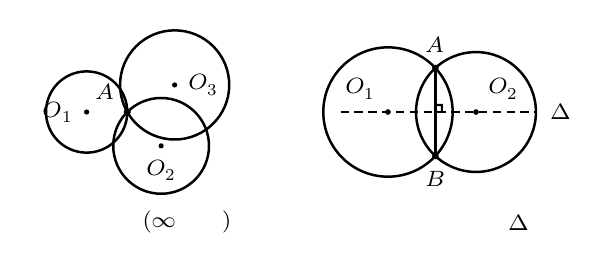
\begin{tikzpicture}[scale=0.86, every node/.style={font=\footnotesize, text=black}]
  % ករណី ១៖ ចំណុច A តែមួយ
  \begin{scope}[shift={(0,0)}]
    \coordinate (A) at (1.25,1.05);
    \coordinate (O1) at (0.65,1.05);
    \coordinate (O2) at (1.75,0.55);
    \coordinate (O3) at (1.95,1.45);
    \draw[black, line width=0.9pt] (O1) circle (0.60);
    \draw[black, line width=0.9pt] (O2) circle (0.707);
    \draw[black, line width=0.9pt] (O3) circle (0.806);
    \fill[black] (A) circle (1.5pt) node[above left=1pt] {$A$};
    \fill[black] (O1) circle (1.1pt) node[left=1.5pt] {$O_1$};
    \fill[black] (O2) circle (1.1pt) node[below=1.5pt] {$O_2$};
    \fill[black] (O3) circle (1.1pt) node[right=1.5pt] {$O_3$};
    \node at (1.35,-0.58) {ករណី ១៖ ១ ចំណុច ($\infty$ រង្វង់)};
  \end{scope}
  % ករណី ២៖ ២ ចំណុច A, B
  \begin{scope}[shift={(4.25,0)}]
    \coordinate (A) at (1.55,1.70);
    \coordinate (B) at (1.55,0.40);
    \coordinate (M) at (1.55,1.05);
    \coordinate (O1) at (0.85,1.05);
    \coordinate (O2) at (2.15,1.05);
    \draw[black, line width=0.85pt, densely dashed] (0.15,1.05) -- (3.05,1.05) node[right=1pt] {$\Delta$};
    \draw[black, line width=1.0pt] (A) -- (B);
    \rightbox[0.16]{A}{M}{O2}
    \draw[black, line width=0.9pt] (O1) circle (0.955);
    \draw[black, line width=0.9pt] (O2) circle (0.885);
    \fill[black] (A) circle (1.4pt) node[above=2pt] {$A$};
    \fill[black] (B) circle (1.4pt) node[below=2pt] {$B$};
    \fill[black] (O1) circle (1.2pt) node[above left=1pt] {$O_1$};
    \fill[black] (O2) circle (1.2pt) node[above right=1pt] {$O_2$};
    \node at (1.60,-0.58) {ករណី ២៖ ផ្ចិតលើមេដ្យាទ័រ $\Delta$};
  \end{scope}
\end{tikzpicture}}

% ៤. E2 Explore: ករណីប្រៀបធៀប ៣ ចំណុចមិនរត់ត្រង់ជួរ vs ៣ ចំណុចរត់ត្រង់ជួរ
\newcommand{\figExploreThreeFourCIRC}{%
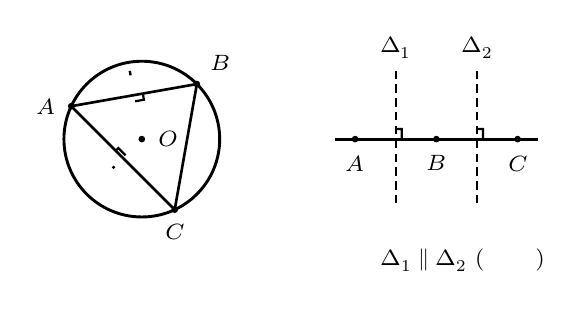
\begin{tikzpicture}[scale=0.86, every node/.style={font=\footnotesize, text=black}]
  % ករណី ៣៖ ៣ ចំណុចមិនរត់ត្រង់ជួរ -> ១ រង្វង់គត់
  \begin{scope}[shift={(0,0)}]
    \coordinate (O) at (1.55,1.05);
    \pgfmathsetmacro{\R}{1.15}
    \coordinate (A) at ($(O)+(155:\R)$);
    \coordinate (B) at ($(O)+(45:\R)$);
    \coordinate (C) at ($(O)+(-65:\R)$);
    \coordinate (Mab) at ($(A)!0.5!(B)$);
    \coordinate (Mac) at ($(A)!0.5!(C)$);
    \draw[black, line width=1.05pt] (O) circle (\R);
    \draw[black, line width=0.95pt] (A) -- (B) -- (C) -- cycle;
    \draw[black, line width=0.85pt, densely dashed] ($(Mab)!-0.45!(O)$) -- ($(O)!1.55!(Mab)$);
    \draw[black, line width=0.85pt, densely dashed] ($(Mac)!-0.45!(O)$) -- ($(O)!1.55!(Mac)$);
    \rightbox[0.14]{B}{Mab}{O}
    \rightbox[0.14]{A}{Mac}{O}
    \fill[black] (A) circle (1.4pt) node[left=2pt] {$A$};
    \fill[black] (B) circle (1.4pt) node[above right=1.5pt] {$B$};
    \fill[black] (C) circle (1.4pt) node[below=1.5pt] {$C$};
    \fill[black] (O) circle (1.4pt) node[right=2.5pt] {$O$};
    \node at (1.55,-0.74) {ករណី ៣៖ រង្វង់តែ ១ គត់};
  \end{scope}
  % ករណី ៤៖ ៣ ចំណុចរត់ត្រង់ជួរ -> មេដ្យាទ័រស្របគ្នា (០ រង្វង់)
  \begin{scope}[shift={(4.25,0)}]
    \draw[black, line width=1.05pt] (0.15,1.05) -- (3.15,1.05);
    \coordinate (A) at (0.45,1.05);
    \coordinate (B) at (1.65,1.05);
    \coordinate (C) at (2.85,1.05);
    \coordinate (I1) at (1.05,1.05);
    \coordinate (I2) at (2.25,1.05);
    \draw[black, line width=0.9pt, densely dashed] (1.05,0.10) -- (1.05,2.05) node[above=1pt] {$\Delta_1$};
    \draw[black, line width=0.9pt, densely dashed] (2.25,0.10) -- (2.25,2.05) node[above=1pt] {$\Delta_2$};
    \rightbox[0.15]{B}{I1}{1.05,2.05}
    \rightbox[0.15]{C}{I2}{2.25,2.05}
    \fill[black] (A) circle (1.4pt) node[below=2.5pt] {$A$};
    \fill[black] (B) circle (1.4pt) node[below=2.5pt] {$B$};
    \fill[black] (C) circle (1.4pt) node[below=2.5pt] {$C$};
    \node at (1.65,-0.74) {ករណី ៤៖ $\Delta_1 \parallel \Delta_2$ (០ រង្វង់)};
  \end{scope}
\end{tikzpicture}}

% ៥. E3 Explain: និយមន័យធាតុនៃរង្វង់ C(O,r) (ទំ.១៩៧)
\newcommand{\figDefCIRC}{%
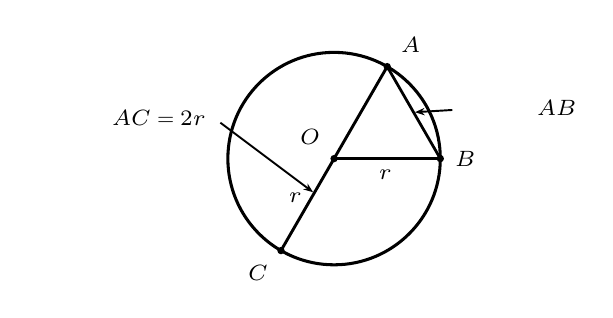
\begin{tikzpicture}[scale=0.95, every node/.style={font=\footnotesize, text=black}]
  \coordinate (O) at (0,0);
  \pgfmathsetmacro{\R}{1.42}
  \coordinate (A) at (60:\R);
  \coordinate (C) at (240:\R);
  \coordinate (B) at (0:\R);
  \draw[black, line width=1.1pt] (O) circle (\R);
  \draw[black, line width=1.05pt] (A) -- (C);
  \draw[black, line width=1.0pt] (A) -- (B) (O) -- (B);
  \fill[black] (O) circle (1.4pt) node[above left=1.5pt] {$O$};
  \fill[black] (A) circle (1.4pt) node[above right=1.5pt] {$A$};
  \fill[black] (C) circle (1.4pt) node[below left=1.5pt] {$C$};
  \fill[black] (B) circle (1.4pt) node[right=2pt] {$B$};
  \node at (0.68,-0.22) {$r$};
  \node at (-0.52,-0.52) {$r$};
  \node[left=2pt] at (-1.52,0.55) {អង្កត់ផ្ចិត $AC=2r$};
  \draw[black, line width=0.7pt, -{Stealth[length=3.5pt]}] (-1.52,0.48) -- (-0.28,-0.45);
  \node[right=2pt] at (1.58,0.68) {អង្កត់ធ្នូ $AB$};
  \draw[black, line width=0.7pt, -{Stealth[length=3.5pt]}] (1.58,0.65) -- (1.08,0.62);
\end{tikzpicture}}

% ៦. E4 Elaborate: លំហាត់គំរូ (ទំ.១៩៨) — មេដ្យាទ័រ MN ⊥ AC និង PQ ⊥ AB កាត់គ្នាត្រង់ O
\newcommand{\figModelCIRC}{%
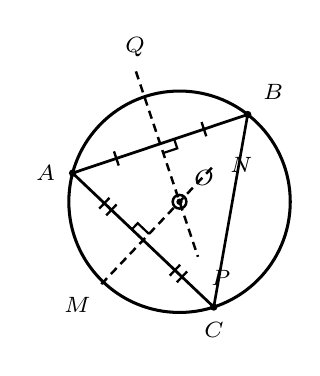
\begin{tikzpicture}[scale=0.95, every node/.style={font=\footnotesize, text=black}]
  \coordinate (O) at (0,0);
  \pgfmathsetmacro{\R}{1.48}
  \coordinate (A) at (165:\R);
  \coordinate (B) at (52:\R);
  \coordinate (C) at (-72:\R);
  \coordinate (Iac) at ($(A)!0.5!(C)$);
  \coordinate (Iab) at ($(A)!0.5!(B)$);
  \draw[black, line width=1.1pt] (O) circle (\R);
  \draw[black, line width=1.0pt, tk1] (A) -- (Iab);
  \draw[black, line width=1.0pt, tk1] (Iab) -- (B);
  \draw[black, line width=1.0pt, tk2] (A) -- (Iac);
  \draw[black, line width=1.0pt, tk2] (Iac) -- (C);
  \draw[black, line width=0.95pt] (B) -- (C);
  % មេដ្យាទ័រ MN (កែង AC) និង PQ (កែង AB) ឆ្លងកាត់ O ទៅសងខាងរង្វង់
  \draw[black, line width=0.9pt, densely dashed] ($(O)!2.15!(Iac)$) node[below left=1pt] {$M$} -- ($(O)!-0.95!(Iac)$) node[right=2pt] {$N$};
  \draw[black, line width=0.9pt, densely dashed] ($(O)!2.25!(Iab)$) node[above=1.5pt] {$Q$} -- ($(O)!-0.95!(Iab)$) node[below right=1pt] {$P$};
  \rightbox[0.16]{A}{Iac}{O}
  \rightbox[0.16]{B}{Iab}{O}
  \fill[black] (A) circle (1.4pt) node[left=2.5pt] {$A$};
  \fill[black] (B) circle (1.4pt) node[above right=2pt] {$B$};
  \fill[black] (C) circle (1.4pt) node[below=2pt] {$C$};
  \draw[black, line width=0.9pt] (O) circle (2.6pt);
  \fill[black] (O) circle (1.2pt) node[above right=2pt] {$O$};
\end{tikzpicture}}

% ៧. E5 Evaluate: ប្រតិបត្តិ (ទំ.១៩៨) — រង្វង់ពីរលើ AB = 6 cm (ករណី ក និង ខ មិនជាន់គ្នា)
\newcommand{\figPracticeCIRC}{%
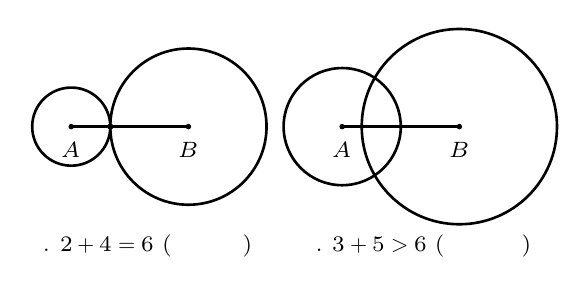
\begin{tikzpicture}[scale=0.62, every node/.style={font=\footnotesize, text=black}]
  % ក. r1=2, r2=4 (ប៉ះគ្នាក្រៅ)
  \begin{scope}[shift={(0,0)}]
    \coordinate (A) at (0,0);
    \coordinate (B) at (2.4,0);
    \draw[black, line width=0.95pt] (A) circle (0.8);
    \draw[black, line width=0.95pt] (B) circle (1.6);
    \draw[black, line width=0.9pt] (A) -- (B);
    \fill[black] (A) circle (1.6pt) node[below=2pt] {$A$};
    \fill[black] (B) circle (1.6pt) node[below=2pt] {$B$};
    \fill[black] (0.8,0) circle (1.8pt);
    \node at (1.5,-2.45) {ក. $2+4=6$ (ប៉ះ ១ ចំណុច)};
  \end{scope}
  % ខ. r1=3, r2=5 (កាត់គ្នា ២ ចំណុច)
  \begin{scope}[shift={(5.55,0)}]
    \coordinate (A) at (0,0);
    \coordinate (B) at (2.4,0);
    \draw[black, line width=0.95pt] (A) circle (1.2);
    \draw[black, line width=0.95pt] (B) circle (2.0);
    \draw[black, line width=0.9pt] (A) -- (B);
    \fill[black] (A) circle (1.6pt) node[below=2pt] {$A$};
    \fill[black] (B) circle (1.6pt) node[below=2pt] {$B$};
    \node at (1.6,-2.45) {ខ. $3+5>6$ (កាត់ ២ ចំណុច)};
  \end{scope}
\end{tikzpicture}}

% ៨. កិច្ចការផ្ទះ៖ លំហាត់ទី៦ និង ទី៧ (ទំ.២០៤)
\newcommand{\figHWCIRC}{%
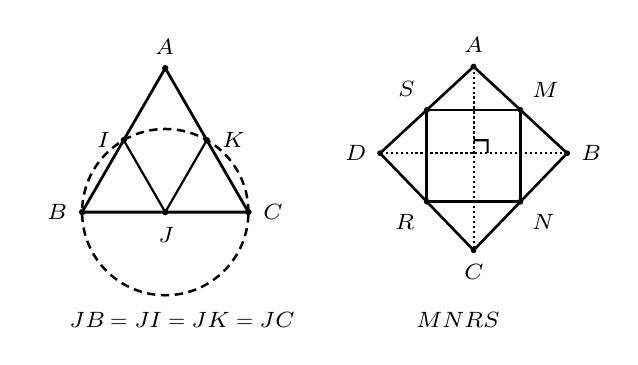
\begin{tikzpicture}[scale=0.88, every node/.style={font=\footnotesize, text=black}]
  % ទី៦៖ ត្រីកោណសម័ង្ស ABC (I, J, K ចំណុចកណ្ដាល -> B, I, K, C លើ C(J, BC/2))
  \begin{scope}[shift={(0,0)}]
    \coordinate (B) at (0,0);
    \coordinate (C) at (2.4,0);
    \coordinate (A) at (1.2,2.078);
    \coordinate (I) at ($(A)!0.5!(B)$);
    \coordinate (J) at ($(B)!0.5!(C)$);
    \coordinate (K) at ($(A)!0.5!(C)$);
    \draw[black, line width=1.0pt] (A) -- (B) -- (C) -- cycle;
    \draw[black, line width=0.9pt, densely dashed] (J) circle (1.2);
    \draw[black, line width=0.8pt] (J) -- (I) (J) -- (K);
    \fill[black] (A) circle (1.3pt) node[above=1.5pt] {$A$};
    \fill[black] (B) circle (1.3pt) node[left=2pt] {$B$};
    \fill[black] (C) circle (1.3pt) node[right=2pt] {$C$};
    \fill[black] (I) circle (1.3pt) node[left=2pt] {$I$};
    \fill[black] (J) circle (1.3pt) node[below=2pt] {$J$};
    \fill[black] (K) circle (1.3pt) node[right=2pt] {$K$};
    \node at (1.2,-1.55) {ទី៦៖ $JB=JI=JK=JC$};
  \end{scope}
  % ទី៧៖ ចតុកោណ ABCD អង្កត់ទ្រូងកែងគ្នា -> M,N,R,S ចតុកោណកែង
  \begin{scope}[shift={(4.45,0)}]
    \coordinate (A) at (1.2,2.10);
    \coordinate (C) at (1.2,-0.55);
    \coordinate (B) at (2.55,0.85);
    \coordinate (D) at (-0.15,0.85);
    \coordinate (M) at ($(A)!0.5!(B)$);
    \coordinate (N) at ($(B)!0.5!(C)$);
    \coordinate (R) at ($(C)!0.5!(D)$);
    \coordinate (S) at ($(D)!0.5!(A)$);
    \draw[black, line width=0.95pt] (A) -- (B) -- (C) -- (D) -- cycle;
    \draw[black, line width=0.8pt, densely dotted] (A) -- (C) (B) -- (D);
    \draw[black, line width=1.0pt] (M) -- (N) -- (R) -- (S) -- cycle;
    \rightbox[0.15]{A}{1.2,0.85}{B}
    \fill[black] (A) circle (1.2pt) node[above=1.5pt] {$A$};
    \fill[black] (B) circle (1.2pt) node[right=1.5pt] {$B$};
    \fill[black] (C) circle (1.2pt) node[below=1.5pt] {$C$};
    \fill[black] (D) circle (1.2pt) node[left=1.5pt] {$D$};
    \fill[black] (M) circle (1.2pt) node[above right=1pt] {$M$};
    \fill[black] (N) circle (1.2pt) node[below right=1pt] {$N$};
    \fill[black] (R) circle (1.2pt) node[below left=1pt] {$R$};
    \fill[black] (S) circle (1.2pt) node[above left=1pt] {$S$};
    \node at (1.2,-1.55) {ទី៧៖ $MNRS$ ចតុកោណកែង};
  \end{scope}
\end{tikzpicture}}

% ============================================================================
% ចាប់ផ្ដើមឯកសារ (Document Body)
% ============================================================================
\begin{document}
\fontsize{10pt}{15.2pt}\selectfont

% -------------------- ក្បាលកិច្ចតែងការ (Header) --------------------
\begin{center}
  {\muol\fontsize{11pt}{16pt}\selectfont ព្រះរាជាណាចក្រកម្ពុជា}\\[2pt]
  {\muol\fontsize{10pt}{15pt}\selectfont ជាតិ សាសនា ព្រះមហាក្សត្រ}\\[1pt]
  \khmflourish
\end{center}

\vspace{-28pt}
{\muol\fontsize{9.5pt}{12.5pt}\selectfont
មន្ទីរអប់រំ យុវជន និងកីឡា ខេត្តកំពង់ធំ\\
ការិយាល័យអប់រំ យុវជន និងកីឡា ស្រុកកំពង់ស្វាយ\\
អនុវិទ្យាល័យព្រះក្រសាំង}

\vspace{1pt}
\begin{center}
  {\muol\fontsize{10pt}{14pt}\selectfont កិច្ចតែងការបង្រៀន}
\end{center}
\vspace{0pt}

% -------------------- ព័ត៌មានទូទៅ (Metadata) --------------------
{\renewcommand{\arraystretch}{0.95}
\hspace*{4.05cm}%
\begin{tabular}{@{}l l l@{}}
  - \hspace{0.35cm} មុខវិជ្ជា & : & គណិតវិទ្យា ថ្នាក់ទី៨ \\
  - \hspace{0.35cm} ចំណងជើងមេរៀន & : & មេរៀនទី១៥ រង្វង់ \\
  - \hspace{0.35cm} ចំណងជើងរង & : & ១. រង្វង់ (និយមន័យ និងការកំណត់រង្វង់ ទំ.១៩៧--១៩៨) \\
  - \hspace{0.35cm} រយៈពេល & : & ១ ម៉ោងសិក្សា (៥០ នាទី) \\
  - \hspace{0.35cm} បង្រៀនដោយ & : & ហុក ប៊ុនថែន \\
  - \hspace{0.35cm} កាលបរិច្ឆេទ & : & ថ្ងៃចន្ទ ទី១៤ ខែធ្នូ ឆ្នាំ២០២៦ \\
\end{tabular}

\vspace{1pt}

% -------------------- I. វត្ថុបំណង --------------------
\textbf{I.} {\muol វត្ថុបំណង}\\[1pt]
\hspace*{0.55cm}%
\begin{tabular}{@{}l l L{14.2cm}@{}}
  \wcirc \hspace{0.25cm} វិជ្ជាសម្បទា & : & សិស្សប្រាប់និយមន័យរង្វង់ $C(O,r)$ អង្កត់កាំ អង្កត់ធ្នូ អង្កត់ផ្ចិត ($d=2r$) និងពោលទ្រឹស្ដីបទការកំណត់រង្វង់តែមួយគត់កាត់តាមបីចំណុចមិនស្ថិតលើបន្ទាត់តែមួយបានត្រឹមត្រូវ ។ \\
  \wcirc \hspace{0.25cm} បំណិនសម្បទា & : & សិស្សសង់និងកំណត់ផ្ចិតរង្វង់តាមប្រសព្វមេដ្យាទ័រលើសន្លឹកកិច្ចការករណីប្រៀបធៀបទាំង ៤ (១ ចំណុច, ២ ចំណុច, ៣ ចំណុចមិនរត់ត្រង់ជួរ, ៣ ចំណុចរត់ត្រង់ជួរ) ស្រាយបញ្ជាក់ $OA=OB=OC$ និងកំណត់ទីតាំងរង្វង់ពីរលើ $AB=6\unit{cm}$ បានត្រឹមត្រូវ ។ \\
  \wcirc \hspace{0.25cm} ចរិយាសម្បទា & : & សិស្សមានទម្លាប់សហការពិភាក្សាជាដៃគូ ផ្ទៀងផ្ទាត់អំណះអំណាងធរណីមាត្រដោយហ្មត់ចត់ និងស្គាល់តម្លៃនៃការរកចំណុចស្មើចម្ងាយក្នុងជីវភាពរស់នៅជាក់ស្ដែង ។ \\
\end{tabular}

\vspace{1pt}

% -------------------- II. សម្ភារៈឧបទេស --------------------
\textbf{II.} {\muol សម្ភារៈឧបទេស}\\[1pt]
\hspace*{0.55cm}$\bullet$ \hspace{0.35cm} សៀវភៅសិក្សាគោលថ្នាក់ទី៨ (ទំ.១៩៧--១៩៨, ២០៤) ក្ដារខៀន ដីស បន្ទាត់ក្រិត កែង និងដែកឈានក្ដារខៀន ព្រមទាំង\textbf{សន្លឹកកិច្ចការសិស្ស ស-ខ្មៅ (\en{Worksheet\_CIRC1} ទំព័រ ១--២)} (បង្រៀនដោយគ្មានស្លាយ \en{LCD})

\vspace{1pt}

% -------------------- III. វិធីសាស្រ្តបង្រៀន --------------------
\textbf{III.} {\muol វិធីសាស្រ្តបង្រៀន}\\[1pt]
\hspace*{0.45cm}%
\begin{tabular}{@{}l l L{14.85cm}@{}}
  $\bullet$ \hspace{0.25cm} គោលវិធី & : & សិស្សមជ្ឈមណ្ឌល (ផ្អែកលើសន្លឹកកិច្ចការរុករក ស-ខ្មៅ ជាគោល គ្មានស្លាយ \en{LCD}) \\
  $\bullet$ \hspace{0.25cm} យុទ្ធវិធីបង្រៀន & : & គំរូ 5Es រួមផ្សំវិធីសាស្ត្រករណីប្រៀបធៀប (\en{Contrasting Cases} \& \en{Variation Theory}) សម្រាយបញ្ជាក់បន្ថយជំនួយ ធនាគារហេតុផល \cnum{1}--\cnum{5} និង \textbf{[tracing]} \\
\end{tabular}
}

\vspace{1pt}

% -------------------- IV. ដំណើរការបង្រៀន --------------------
\textbf{IV.} {\muol ដំណើរការបង្រៀន}

\vspace{1pt}

\renewcommand{\arraystretch}{1.15}
\begin{longtable}{|L{5.50cm}|L{7.90cm}|L{4.80cm}|}
\hline
\rowcolor{headgray}
\multicolumn{1}{|c|}{\muol សកម្មភាពគ្រូ} &
\multicolumn{1}{c|}{\muol ខ្លឹមសារមេរៀន} &
\multicolumn{1}{c|}{\muol សកម្មភាពសិស្ស} \\
\hline
\endfirsthead

\hline
\endhead

\hline
\endfoot

\hline
\endlastfoot

% ==================== ជំហានទី១ (2min) ====================
\stepheader{ជំហានទី១ \enbf{(}រដ្ឋបាលថ្នាក់\enbf{)}}
$\bullet$ ពិនិត្យអវត្តមាន សណ្ដាប់ធ្នាប់ អនាម័យ និងឧបករណ៍សិក្សា (បន្ទាត់ក្រិត កែង ដែកឈាន)
&
$\bullet$ រដ្ឋបាលថ្នាក់ និងការត្រៀមសម្ភារៈគូសវាស់លើសន្លឹកកិច្ចការ
&
$\circ$ ប្រធានថ្នាក់រាយការណ៍អវត្តមាន និងត្រៀមបន្ទាត់ ដែកឈាន \\[3pt]

$\bullet$ ចាត់សិស្សជាគូ/ក្រុម ៣ នាក់ និងចែក \textbf{សន្លឹកកិច្ចការ ១៥.១} (ទំព័រ ១--២) ផ្កាប់លើតុ
&
$\bullet$ ក្រុមសិក្សាស្រាវជ្រាវតាមសន្លឹកកិច្ចការ ស-ខ្មៅ
&
$\circ$ អង្គុយតាមក្រុម និងដាក់សន្លឹកកិច្ចការផ្កាប់លើតុ \\
\hline

% ==================== ជំហានទី២ (9min: <=3 + 3 + E1 3) ====================
\stepheader{ជំហានទី២ \enbf{(}ពិនិត្យចំណេះដឹងមុន \enbf{+} ទំនាក់ទំនងមេរៀនថ្មី\enbf{)}}
\ditem \textbf{ពិនិត្យកិច្ចការមេរៀនមុន ($\le 3\unit{min}$)} \timenote{កុំសរសេរវែងលើក្ដារ} \par
$\bullet$ សួរផ្ទាល់មាត់រំលឹកពហុកោណនិយ័ត (មេរៀនទី១៤) និងចម្ងាយពីផ្ចិតទៅកំពូលទាំងអស់
&
{\centering\redsub{ការភ្ជាប់ពីមេរៀនទី១៤ មកមេរៀនទី១៥}\par} \par
$\bullet$ ក្នុងពហុកោណនិយ័ត ផ្ចិត $O$ មានចម្ងាយស្មើៗគ្នាទៅគ្រប់កំពូល ($OA=OB=OC=\dots=r$) ។
&
$\circ$ ឆ្លើយផ្ទាល់មាត់៖ «ចម្ងាយពីផ្ចិតទៅគ្រប់កំពូលស្មើៗគ្នា!» \\[3pt]

\ditem \textbf{រំលឹកមេរៀនទាក់ទង (3min)} \timenote{សរុបកុំឱ្យលើស 3min} \par
$\bullet$ គូសអង្កត់ $AB$ និងមេដ្យាទ័រ $\Delta$ លើក្ដារខៀន
&
{\centering\redsub{រំលឹកលក្ខណៈមេដ្យាទ័រនៃអង្កត់}\par} \par
$\bullet$ បន្ទាត់ $\Delta$ កែងនឹង $AB$ ត្រង់ចំណុចកណ្ដាល $I$ ហៅថា\textbf{មេដ្យាទ័រ}នៃ $AB$ ។
&
$\circ$ សង្កេតអង្កត់ $AB$ និងមេដ្យាទ័រ $\Delta$ លើក្ដារខៀន \\[3pt]

– \textbf{សំណួរ៖} តើចំណុច $M$ ស្ថិតលើមេដ្យាទ័រ $\Delta$ នៃ $AB$ មានលក្ខណៈដូចម្ដេច?
&
$\bullet$ \graybox{$M \in \Delta \iff MA = MB$} (គ្រប់ចំណុចស្មើចម្ងាយពី $A, B$ ស្ថិតលើ $\Delta$) ។
&
$\circ$ ឆ្លើយ៖ «$MA = MB$ ហើយបើ $MA=MB$ នោះ $M\in\Delta$!» \\[3pt]

&
\cfig{\figPrereqCIRC}
& \\[3pt]

\fiveE{E1 - Engage (3min)} \timenote{(កុំទាន់ផ្ដល់ចម្លើយ)} \par
\ditem \textbf{បញ្ហាជីវភាពពិត (ស្រុកកំពង់ស្វាយ)៖} \par
គូសប្លង់ភូមិ $A, B, C$ ពីរទម្រង់លើក្ដារខៀន (ទម្រង់ត្រីកោណ និងទម្រង់រត់ត្រង់ជួរតាមផ្លូវជាតិ)
&
{\centering\redsub{បេសកកម្ម៖ ជ្រើសទីតាំងអណ្ដូងទឹកស្អាតរួម $O$}\par}
&
$\circ$ សង្កេតប្លង់ភូមិទាំងពីរលើក្ដារខៀន និងផ្នែកក្បាលសន្លឹកកិច្ចការ \\[3pt]

&
\cfig{\figEngageCIRC}
& \\[3pt]

– \textbf{សំណួរ (ក)៖} បើភូមិ $A, B, C$ មិនរត់ត្រង់ជួរ តើអាចជីកអណ្ដូងរួម $O$ ($OA=OB=OC$) បានប៉ុន្មានកន្លែង?
&
\textbf{ចម្ងល់គោល (ក)៖} ករណី $A, B, C$ មិនរត់ត្រង់ជួរ $\to$ មានរង្វង់ប៉ុន្មានកាត់តាម $A,B,C$?
&
$\circ$ ពិភាក្សាទស្សន៍ទាយក្នុងក្រុមលើសំណួរ (ក) \\[3pt]

– \textbf{សំណួរ (ខ)៖} ចុះបើភូមិទាំង ៣ រត់ត្រង់ជួរតាមបណ្ដោយផ្លូវត្រង់ តើរកឃើញចំណុច $O$ ស្មើចម្ងាយដែរឬទេ?
&
\textbf{ចម្ងល់គោល (ខ)៖} ករណី $A, B, C$ រត់ត្រង់ជួរ $\to$ មានរង្វង់កាត់តាមទាំងបីឬទេ?
&
$\circ$ កត់ចម្លើយទាយជាមុនលើផ្នែកក្បាលសន្លឹកកិច្ចការ \\
\hline

% ==================== ជំហានទី៣ (17min: E2 11m + E3 6m) ====================
\stepheader{ជំហានទី៣ \enbf{(}ខ្លឹមសារមេរៀនថ្មី\enbf{)}}
\fiveE{E2 - Explore (11min)} \par
$\bullet$ សរសេរចំណងជើងមេរៀនលើក្ដារខៀន និងឱ្យសិស្សបើក \textbf{សន្លឹកកិច្ចការ ទំព័រ ១ (ផ្នែក ក)}
&
មេរៀនទី១៥ \hspace{0.15cm} {\muol រង្វង់} \par
១. រង្វង់ (និយមន័យ និងការកំណត់រង្វង់)
&
$\circ$ កត់ចំណងជើងមេរៀន និងបើកសន្លឹកកិច្ចការទំព័រ ១ \\[3pt]

\ditem \textbf{សកម្មភាពរុករកតាមករណីប្រៀបធៀបទាំង ៤ (\en{Contrasting Cases})} \par
$\bullet$ \textbf{ជំហានទី១ក (2.5min)៖} ឱ្យក្រុមសិស្សគូសរង្វង់កាត់តាមចំណុច $A$ តែមួយ លើប្រអប់ \textbf{ករណីទី១}
&
{\centering\textbf{ការរកឃើញករណីទី១ និង ករណីទី២ (លើសន្លឹកកិច្ចការទំព័រ ១)}\par} \par
$\bullet$ \textbf{ករណីទី១ (១ ចំណុច $A$)៖} គូសរង្វង់ផ្ចិត $O_1, O_2, O_3\dots$ កាត់តាម $A$ បាន\textbf{ច្រើនរាប់មិនអស់} (ផ្ចិតស្ថិតក្នុងប្លង់) ។
&
$\circ$ ប្រើដែកឈានគូសរង្វង់ផ្ចិត $O_2, O_3$ កាត់តាមចំណុច $A$ \\[3pt]

$\bullet$ \textbf{ជំហានទី១ខ (2.5min)៖} ឱ្យសិស្សសង់មេដ្យាទ័រ $\Delta$ នៃ $AB$ ($3.0\unit{cm}$) និងគូសរង្វង់លើប្រអប់ \textbf{ករណីទី២}
&
$\bullet$ \textbf{ករណីទី២ (២ ចំណុច $A, B$)៖} ព្រោះ $OA=OB$ ផ្ចិតទាំងអស់ត្រូវស្ថិតលើ\textbf{មេដ្យាទ័រ $\Delta$ នៃ $AB$} $\Rightarrow$ គូសបាន\textbf{ច្រើនរាប់មិនអស់} ។
&
$\circ$ សង់មេដ្យាទ័រ $\Delta$ នៃ $AB$ និងវាស់ផ្ទៀង $O_1A = O_1B$ \\[3pt]

&
\cfig{\figExploreOneTwoCIRC}
& \\[3pt]

$\bullet$ \textbf{ជំហានទី២ក (3min)៖} ឱ្យសិស្សគូសបន្តមេដ្យាទ័រ $\Delta_1, \Delta_2$ រកប្រសព្វ $O$ លើ \textbf{ករណីទី៣} ($A,B,C$ មិនរត់ត្រង់ជួរ)
&
$\bullet$ \textbf{ករណីទី៣ ($A,B,C$ មិនរត់ត្រង់ជួរ)៖} មេដ្យាទ័រនៃជ្រុង $\tri{ABC}$ កាត់គ្នាត្រង់ \graybox{ចំណុច $O$ តែមួយគត់} ($OA=OB=OC$) $\Rightarrow$ គូសបាន\textbf{រង្វង់តែមួយគត់} ។
&
$\circ$ គូសមេដ្យាទ័ររកប្រសព្វ $O$ និងវាស់ផ្ទៀង $OA=OB=OC$ \\[3pt]

$\bullet$ \textbf{ជំហានទី២ខ (3min)៖} ប្រៀបធៀបនឹង \textbf{ករណីទី៤} ($A,B,C$ រត់ត្រង់ជួរ) \par
– \textbf{សំណួរ៖} ហេតុអ្វីករណីទី៤ មេដ្យាទ័រទាំងពីរមិនជួបគ្នា?
&
$\bullet$ \textbf{ករណីទី៤ ($A,B,C$ រត់ត្រង់ជួរ)៖} $\Delta_1 \perp AC$ និង $\Delta_2 \perp AC \Rightarrow \Delta_1 \parallel \Delta_2$ (គ្មានចំណុចប្រសព្វ) $\Rightarrow$ \graybox{គូសមិនបានរង្វង់ទេ (០ រង្វង់)}!
&
$\circ$ សង្កេតឃើញ $\Delta_1 \parallel \Delta_2$ និងបំពេញតារាងប្រៀបធៀបទាំង ៤ ករណី \\[3pt]

&
\cfig{\figExploreThreeFourCIRC}
& \\[3pt]

% --- E3 Explain (6min) ---
\fiveE{E3 - Explain (6min)} \par
\ditem \textbf{សំយោគនិយមន័យធាតុនៃរង្វង់ (ទំ.១៩៧)} \par
$\bullet$ ឱ្យតំណាងក្រុមបង្ហាញលទ្ធផល រួចគ្រូគូសរង្វង់ $C(O,r)$ លើក្ដារខៀន
&
\textbf{និយមន័យ (ទំ.១៩៧)៖} \textbf{រង្វង់}ផ្ចិត $O$ កាំ $r$ កំណត់ដោយ $C(O,r)$ គឺជាសំណុំគ្រប់ចំណុច $M$ ក្នុងប្លង់ដែលមានចម្ងាយ $OM=r$ ។
&
$\circ$ បំពេញប្រអប់និយមន័យក្នុងសន្លឹកកិច្ចការទំព័រ ១ (ផ្នែក ខ) \\[3pt]

$\bullet$ បញ្ជាក់ភាពខុសគ្នារវាង អង្កត់កាំ អង្កត់ធ្នូ និងអង្កត់ផ្ចិត ($d=2r$) លើក្ដារខៀន
&
$\bullet$ \textbf{អង្កត់កាំ៖} $OA = OB = OC = r$ ។ \par
$\bullet$ \textbf{អង្កត់ធ្នូ៖} អង្កត់ភ្ជាប់ពីរចំណុចនៃរង្វង់ (ឧ. $AB$) ។ \par
$\bullet$ \textbf{អង្កត់ផ្ចិត៖} អង្កត់ធ្នូដែលកាត់តាមផ្ចិត $O$ (ឧ. $AC = 2r$) ។
&
$\circ$ កត់សម្គាល់ធាតុទាំងបីនៃរង្វង់ និងទំនាក់ទំនង $d=2r$ \\[3pt]

&
\cfig{\figDefCIRC}
& \\[3pt]

\ditem \textbf{បង្គុំទ្រឹស្ដីបទការកំណត់រង្វង់ (ទំ.១៩៨)} \par
$\bullet$ សង្ខេបទ្រឹស្ដីបទ និងសម្គាល់ករណីបីចំណុចរត់ត្រង់ជួរ
&
\textbf{ទ្រឹស្ដីបទ (ទំ.១៩៨)៖} តាមបីចំណុចដែលមិនស្ថិតនៅលើបន្ទាត់តែមួយ គេអាចគូសបាន\textbf{រង្វង់តែមួយគត់}ដែលកាត់តាមចំណុចទាំងនោះ ។ \par
\textbf{សម្គាល់៖} បើបីចំណុចស្ថិតលើបន្ទាត់តែមួយ គេមិនអាចគូសរង្វង់កាត់តាមវាទេ ។
&
$\circ$ បំពេញទ្រឹស្ដីបទក្នុងផ្នែក ខ នៃសន្លឹកកិច្ចការ \\[3pt]

$\bullet$ ណែនាំ\textbf{ធនាគារហេតុផល \cnum{1}--\cnum{5}} សម្រាប់យោងក្នុងសម្រាយបញ្ជាក់
&
\textbf{ធនាគារហេតុផល៖} \cnum{1} និយមន័យ $C(O,r)$ ($OM=r$) \textbar{} \cnum{2} មេដ្យាទ័រ ($MA=MB$) \textbar{} \cnum{3} លក្ខណៈឆ្លងស្មើគ្នា \textbar{} \cnum{4} ទ្រឹស្ដីបទ ៣ ចំណុចមិនរត់ត្រង់ជួរ \textbar{} \cnum{5} បន្ទាត់ពីរកែងនឹងបន្ទាត់តែមួយ ($\Delta_1\parallel\Delta_2$) ។
&
$\circ$ អានផ្ទៀងលេខកូដ \cnum{1}--\cnum{5} សម្រាប់ប្រើក្នុង E4 \\
\hline

% ==================== ជំហានទី៤ (20min: E4 10m + E5 10m) ====================
\stepheader{ជំហានទី៤ \enbf{(}ពង្រីកចំណេះដឹង\enbf{)}}
\fiveE{E4 - Elaborate (10min)} \par
\ditem \textbf{លំហាត់គំរូ (ទំ.១៩៨) — សន្លឹកកិច្ចការទំព័រ ២ (ផ្នែក គ)} \par
$\bullet$ ឱ្យសិស្សគូស \textbf{[tracing]} តាមមេដ្យាទ័រ $MN \perp AC$ និង $PQ \perp AB$ ដែលប្រសព្វគ្នាត្រង់ $O$
&
{\muol លំហាត់គំរូ} \textbf{(ទំ.១៩៨)៖} គេមានបីចំណុច $A, B$ និង $C$ មិនស្ថិតលើបន្ទាត់តែមួយ (កំពូលនៃ $\tri{ABC}$) ។ ស្រាយបញ្ជាក់ថា $A, B$ និង $C$ ស្ថិតនៅលើរង្វង់តែមួយ ។
&
$\circ$ បើកសន្លឹកកិច្ចការទំព័រ ២ (ផ្នែក គ) និងគូស \textbf{[tracing]} លើ $MN, PQ$ \\[3pt]

&
\cfig{\figModelCIRC}
& \\[3pt]

$\bullet$ ដឹកនាំសិស្សបំពេញតារាងសម្រាយបញ្ជាក់ជំហាន ១ និង ២ ដោយផ្អែកលើលក្ខណៈមេដ្យាទ័រ (\cnum{2})
&
$\bullet$ \textbf{ជំហាន ១៖} $MN$ ជាមេដ្យាទ័រនៃ $AC$ ហើយ $O\in MN \Rightarrow OA = OC$ (\cnum{2}) ។ \par
$\bullet$ \textbf{ជំហាន ២៖} $PQ$ ជាមេដ្យាទ័រនៃ $AB$ ហើយ $O\in PQ \Rightarrow OA = OB$ (\cnum{2}) ។
&
$\circ$ បំពេញចន្លោះជំហាន ១ និង ២ ព្រមទាំងលេខហេតុផល \cnum{2} \\[3pt]

$\bullet$ ឱ្យសិស្សទាញសន្និដ្ឋានជំហាន ៣--៤ និងឆ្លើយ \textbf{សំណួរ EIA 30s}៖ ហេតុអ្វីមេដ្យាទ័រទី៣ នៃ $BC$ ក៏កាត់តាម $O$ ដែរ?
&
$\bullet$ \textbf{ជំហាន ៣៖} តាមលក្ខណៈឆ្លង បាន \graybox{$OA = OB = OC$} (\cnum{3}) ។ \par
$\bullet$ \textbf{ជំហាន ៤៖} រង្វង់ $C(O,OA)$ កាត់តាម $A, B, C$ តែមួយគត់ (\cnum{1}, \cnum{4}) ។ \par
\timenote{EIA 30s៖ ព្រោះ $OB=OC$ នោះ $O$ ក៏ស្ថិតលើមេដ្យាទ័រនៃ $BC$ ដែរ!}
&
$\circ$ បំពេញជំហាន ៣--៤ និងសរសេរចម្លើយ EIA 30s \\[3pt]

\fiveE{E5 - Evaluate (10min)} \par
\ditem {\muol លំហាត់ប្រតិបត្តិ} \textbf{(6.5min — សន្លឹកកិច្ចការទំព័រ ២ ផ្នែក ឃ)} \par
$\bullet$ ឱ្យសិស្សប្រើដែកឈានសង់ធ្នូរង្វង់លើអង្កត់ខ្នាតពិត $AB=6\unit{cm}$ ក្នុងករណី ក និង ខ
&
{\muol លំហាត់ប្រតិបត្តិ} \textbf{(ទំ.១៩៨)៖} គេឱ្យអង្កត់ $AB = 6\unit{cm}$ ។ គូសរង្វង់៖ \par
$\bullet$ \textbf{ក.} $C(A,2\unit{cm})$ និង $C(B,4\unit{cm})$៖ $2+4 = 6 = AB \Rightarrow$ \textbf{ប៉ះគ្នាក្រៅ (១ ចំណុច)} ។ \par
$\bullet$ \textbf{ខ.} $C(A,3\unit{cm})$ និង $C(B,5\unit{cm})$៖ $5-3 < 6 < 3+5 \Rightarrow$ \textbf{កាត់គ្នា (២ ចំណុច)} ។
&
$\circ$ គូសធ្នូរង្វង់ករណី ក និង ខ លើខ្នាតពិត $AB=6\unit{cm}$ \\[3pt]

$\bullet$ ឱ្យសិស្សគូសករណី គ និងទាញលក្ខខណ្ឌប្រៀបធៀប $r_1+r_2$ ជាមួយ $AB$
&
$\bullet$ \textbf{គ.} $C(A,1\unit{cm})$ និង $C(B,2\unit{cm})$៖ $1+2 = 3 < 6 \Rightarrow$ \textbf{ដាច់ពីគ្នា (០ ចំណុច)} ។
&
$\circ$ បំពេញតារាងចំនួនចំណុចប្រសព្វទាំង ៣ ករណី \\[3pt]

&
\cfig{\figPracticeCIRC}
& \\[3pt]

\ditem \textbf{បិទបញ្ហា E1 និងផ្ទៀងសំណួរវិនិច្ឆ័យ A--D (3.5min — ផ្នែក ង)} \par
$\bullet$ ឱ្យសិស្សឆ្លើយបិទបេសកកម្មអណ្ដូងទឹករួម E1 និងគូសធីកប្រអប់ A--D លើផ្នែកខាងក្រោមសន្លឹកកិច្ចការ
&
$\bullet$ \textbf{បិទ E1៖} (ក) ភូមិ ៣ មិនរត់ត្រង់ជួរ មានទីតាំងអណ្ដូង $O$ \textbf{តែ ១ គត់} (\cnum{4}); (ខ) ភូមិ ៣ រត់ត្រង់ជួរ \textbf{គ្មានទីតាំង $O$ ស្មើចម្ងាយទេ} (\cnum{5}) ។ \par
$\bullet$ \textbf{ចម្លើយរហ័ស A--D៖} A (\ding{55} អង្កត់ធ្នូមិនចាំបាច់កាត់ផ្ចិតទេ) \textbar{} B (\ding{51} ផ្ចិតនៅលើមេដ្យាទ័រ $AB$) \textbar{} C (\ding{55} ៣ ចំណុចរត់ត្រង់ជួរគូសមិនបាន) \textbar{} D (\ding{51} $d=2r=10\unit{cm}$) ។
&
$\circ$ បំពេញប្រអប់ A--D ផ្ទៀងចម្លើយ និងលើកសន្លឹកកិច្ចការបង្ហាញគ្រូ \\
\hline

% ==================== ជំហានទី៥ (<=2min) ====================
\stepheader{ជំហានទី៥ \enbf{(}កិច្ចការផ្ទះ \enbf{+} បណ្ដាំផ្ញើ\enbf{)}}
\timenote{ចំណាយពេលឱ្យតិចបំផុតកុំឱ្យលើស 2min} \par
$\bullet$ ណែនាំកិច្ចការផ្ទះ \textbf{លំហាត់ទី៦ (ទំ.២០៤)} នៅផ្នែកចុងក្រោយនៃសន្លឹកកិច្ចការទំព័រ ២
&
{\centering{\muol កិច្ចការផ្ទះ} \textbf{(សៀវភៅគោល ទំ.២០៤ ៖ លំហាត់ទី៦ និង ទី៧)}\par} \par
$\bullet$ \textbf{លំហាត់ទី៦៖} $\tri{ABC}$ សម័ង្ស; $I,J,K$ ជាចំណុចកណ្ដាលនៃ $AB,BC,CA$ ។ បង្ហាញថា $B,I,K,C$ ស្ថិតលើរង្វង់តែមួយ (\textit{តម្រុយ៖ $JB=JC=JI=JK=\frac{BC}{2}$}) ។
&
$\circ$ កត់ត្រាតម្រុយលំហាត់ទី៦ លើសន្លឹកកិច្ចការ \\[3pt]

$\bullet$ ណែនាំបន្ត \textbf{លំហាត់ទី៧ (ទំ.២០៤)} ឱ្យសិស្សសង់រូបនិងបង្ហាញលក្ខណៈចតុកោណកែងនៅផ្ទះ
&
$\bullet$ \textbf{លំហាត់ទី៧៖} ចតុកោណ $ABCD$ មាន $AC\perp BD$; $M,N,R,S$ ជាចំណុចកណ្ដាលជ្រុងទាំងបួន ។ បង្ហាញថា $M,N,R,S$ ស្ថិតលើរង្វង់តែមួយ (\textit{តម្រុយ៖ $MNRS$ ជាចតុកោណកែង}) ។
&
$\circ$ កត់ត្រាតម្រុយលំហាត់ទី៧ លើសន្លឹកកិច្ចការ \\[3pt]

&
\cfig{\figHWCIRC}
& \\[3pt]

$\bullet$ ផ្ដាំផ្ញើសិស្សអានមេរៀនបន្ត \textbf{២. មុំផ្ចិត និងធ្នូ (ទំ.១៩៩--២០០)} និងរក្សាសុវត្ថិភាពពេលធ្វើដំណើរ
&
$\bullet$ អានជាមុន៖ \textbf{២. មុំផ្ចិត និងធ្នូ} (ទំ.១៩៩--២០០) \par
$\bullet$ បណ្ដាំផ្ញើ និងវិន័យសីលធម៌
&
$\circ$ ទទួលបណ្ដាំផ្ញើ និងជម្រាបលាគ្រូ \\
\end{longtable}

% -------------------- កាលបរិច្ឆេទ និងហត្ថលេខា (Date & Signature) --------------------
\vspace{16pt}
\hfill
\begin{minipage}{9.8cm}
  {\centering
    ថ្ងៃចន្ទ ៥កើត ខែមិគសិរ ឆ្នាំមមី អដ្ឋស័ក ពុទ្ធសករាជ ២៥៧០\\[3pt]
    កំពង់ស្វាយ, ថ្ងៃទី១៤ ខែធ្នូ ឆ្នាំ២០២៦\\[4pt]
    {\muol គ្រូបង្រៀន}\par}
  \vspace{32pt}
  \hfill{\muol ហុក ប៊ុនថែន}\hspace*{1.4cm}
\end{minipage}

\end{document}
